\section{Sesión 1}
\subsection{Método de Euler}
En esta primera sesión vamos a empezar a familiarizarnos con MATLAB (o en su defecto Octave) y a implementar el método de Euler, para después poder realizar algunas comparaciones visuales a fin de comprobar lo efectivo del método.

Vamos a resolver el siguiente problema de valor incial.
\[\left\{\begin{array}{l}
\left( \begin{array}{c}
v_1' \\
v_2'  \end{array} \right)=f(t,v) =\left( \begin{array}{cc}
-2 & 1 \\
1 & -2 \end{array} \right)\left( \begin{array}{c}
v_1 \\
v_2 \end{array} \right) + \left( \begin{array}{c}
2\sin(t) \\
2(\cos(t)-\sin(t))  \end{array} \right)
v(0) = \left( \begin{array}{c}
2 \\
3  \end{array} \right)\end{array}\right.\]

Hemos escogido un sistema que somos capaces de resolver a mano puesto que así podremos comprobar la calidad de la solución obtenida.

En este caso, sabemos de antemano que la solución es:
\[v(t)=\left( \begin{array}{c}
2e^{-t}+\sin(t) \\
2e^{-t}+\cos(t)  \end{array} \right)\]

Vamos ahora a implementarlo en el ordenador. Lo primero que tenemos que hacer es definir las funciones mencionadas anteriormente, es decir, $f(t,v)$ y la solución. Vamos a emplear para ello ficheros distintos (cada fichero con el mismo nombre que la función que estamos definiendo para que MATLAB/Octave pueden encontrar la función) aunque podría hacerse todo en el mismo.

\begin{center}
    \begin{minipage}{0.55\textwidth}
        \centering
        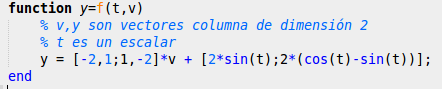
\includegraphics[width=\textwidth]{img/f.png}
    \end{minipage}
    \begin{minipage}{.4\textwidth}
        \centering
        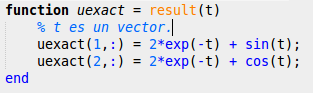
\includegraphics[width=\textwidth]{img/result.png}
    \end{minipage}
\end{center}

Una vez tenemos estas funciones definidas, procedemos a implementar el propio método de Euler, que podemos ver en la siguiente imagen.

\begin{center}
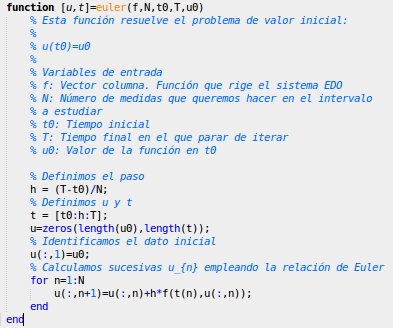
\includegraphics[width=0.6\textwidth]{img/euler.png}
\end{center}

Por último sólo tenemos que crear un programa principal que, llamando a las funciones ya definidas, resuelva el PVI planteado al inicio de esta sección.

\begin{center}
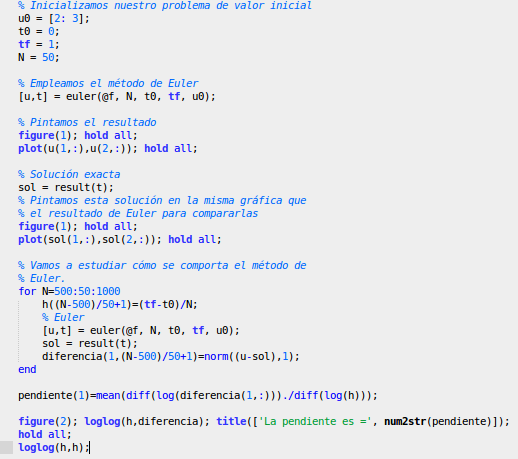
\includegraphics[width=0.8\textwidth]{img/aplicacion_euler.png}
\end{center}

Vamos a explicar detenidamente qué se está haciendo en este código. Para empezar estamos simplemente resolviendo el problema aplicando el método de Euler y pintando, en una misma gráfica, la solución dada por el método y la solución real, con lo que podemos observar la gran precisión de la solución obtenida por este método.
\begin{center}
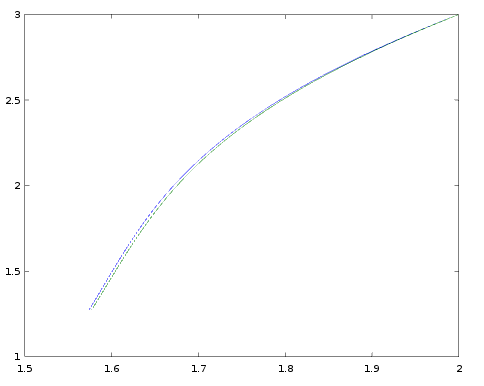
\includegraphics[width=0.8\textwidth]{img/figure1.png}
\end{center}

La última parte del código es la más compleja. Lo qye se está haciendo ahí es llamar numerosas veces al método de Euler y guardar, en cada llamada, la diferencia entre la función obtenida y la solución así como el $h$ empleado en esa ocasión.

Posteriormente calculamos la pendiente de la función que representan los pares de valores que hemos guardado. Para ello tomamos escala logarítmica y estudiamos la pendiente de la función en cada punto para, finalmente, tomar la media de esos valores.

Por último, pintamos estos valores junto con una función claramente lineal, que es $h$ con respecto a $h$ y obtenemos la siguiente gráfica.

\begin{center}
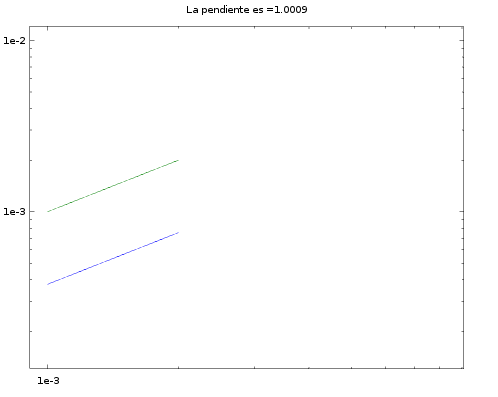
\includegraphics[width=0.8\textwidth]{img/figure2.png}
\end{center}

Ahora la pregunta que nos surge es clara, \textbf{¿por qué es interesante esta pendiente?}.

La idea se basa en el hecho de haber trabajado con logaritmos de los valores y no con los valores directamente. En general sabemos que el error se comporta como $e \leq c h^p$ para una cierta constante $c$, donde $p$ es el orden del método. Evidentemente podemos aplicar logaritmos a ambos lados sin que nada se estropee, obteniendo:
\[\log(e) \leq p \log(ch)\]

Si ahora dibujásemos la gráfica que relaciona el logaritmo del error con el logaritmo de $h$ obtendremos una recta con pendiente $p$ que es justo el \textbf{orden del método}.

Por tanto, esa pendiente que hemos calculado en el código, nos permite conocer el orden del método de Euler.

\section{Sesión 2}
\subsection{Método Runge Kutta de orden 4}
\subsubsection{Explícito}
En esta sesión vamos a implementar un método Runge Kutta explícito. Para ello, recordemos que el método Runge Kutta se basaba en el empleo de las funciones:
\[K_i = f(x_n+c_ih,y_n+\sum_j A_{ij}K_j)\]

En el caso del método Runge Kutta de cuarto orden teníamos:

\[
\begin{array}{ll}
K_1 = & f(x_n,y_n)\\
K_2 = & f(x_n+\frac{h}{2}, y_n+\frac{h}{2}K_1)\\
K_3 = & f(x_n+\frac{h}{2}, y_n + \frac{h}{2}K_2)\\
K_4 = & f(x_n+h, y_n + h K_3)
\end{array}
\]

Si escribimos todas las variables en una tabla (que sería la matriz de las $A_{ij}$ unida a la columna formada por las $c_i$) podemos ver que el método que origina la tabla es explícito si y sólo si no hay ningún elemento no nulo por encima de la diagonal principal.

\obs Queda como ejercicio para el lector la comprobación y el autoconvencimiento de que la afirmación anterior es cierta, pues es algo completamente trivial.

Para implementar el método, lo primero que hacemos es crear un fichero con la función \textit{PKexplicito} cuyo contenido se muestra a continuación
\begin{center}
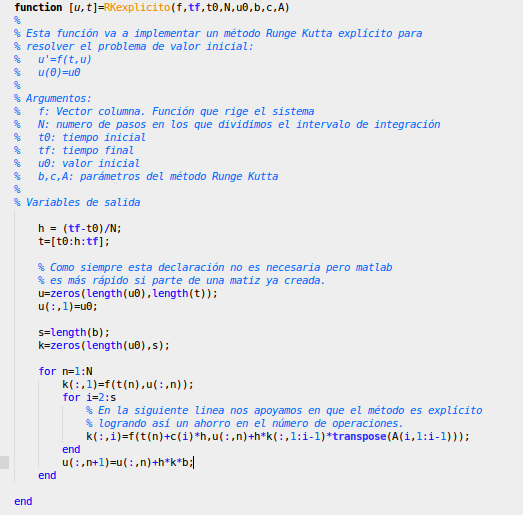
\includegraphics[width=0.6\textwidth]{img/RK4_explicito.png}
\end{center}

Ahora escribimos un pequeño programa que inicializará \textbf{el mismo PVI que ya resolvimos en la sesión de laboratorio anterior} (emplearemos por tanto las mismas funciones $f$ y $result$).
\begin{center}
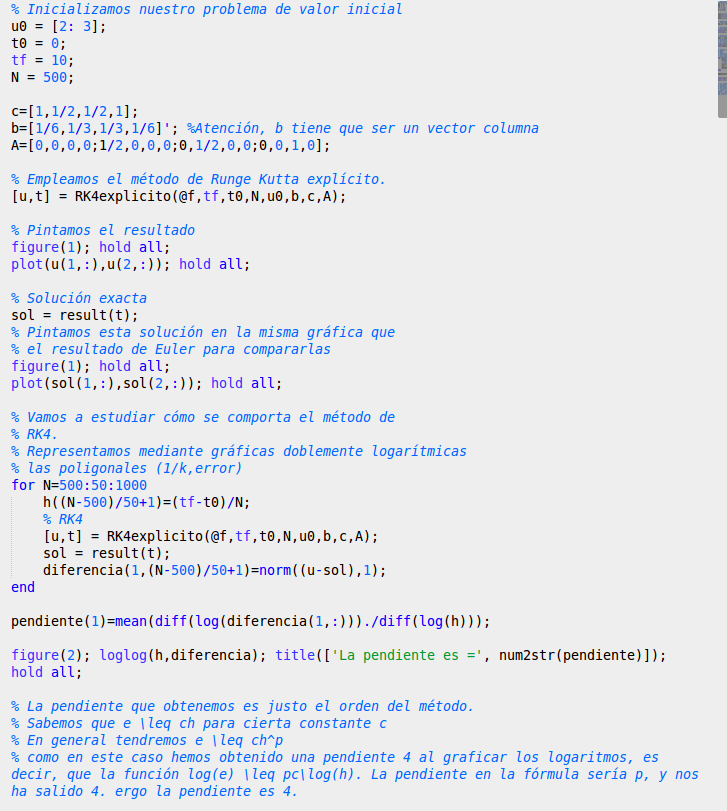
\includegraphics[width=0.6\textwidth]{img/PVI_RK4_explicito.png}
\end{center}

El código es totalmente equivalente al empleado en la sesión anterior, salvo que invocamos el método RK4 en lugar del método de Euler.

Las gráficas obtenidas, que dibujan la función resultado y la obtenida con RK4 por un lado y la relación entre el erro y $h$ en escala logarítmica por otro, son:
\begin{center}
    \begin{minipage}{0.49\textwidth}
        \centering
        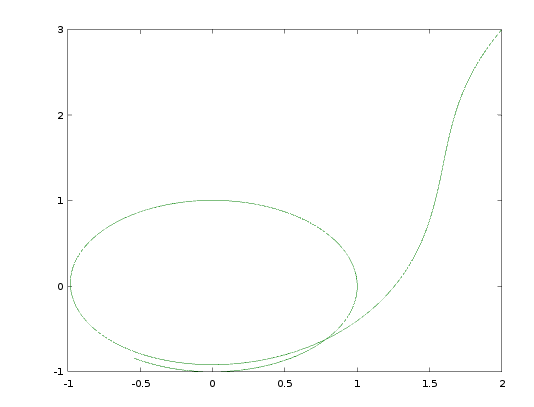
\includegraphics[width=\textwidth]{img/RK4_explicito_grafica.png}
    \end{minipage}
    \begin{minipage}{.49\textwidth}
        \centering
        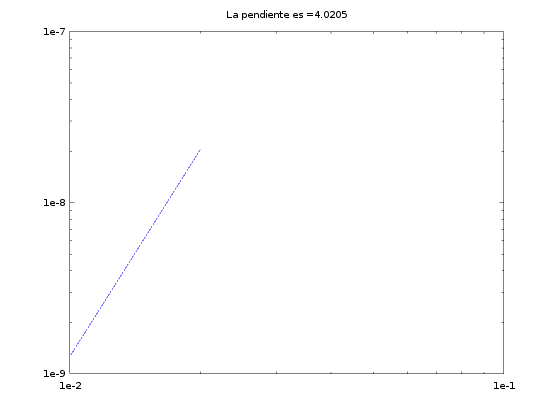
\includegraphics[width=\textwidth]{img/RK4_explicito_pendiente.png}
    \end{minipage}
\end{center}

Y tal y como hemos visto en clase, obtenemos que el método RK4 tiene orden 4.

\obs La diferencia observada entre esta función y la obtenida en la sesión anterior radica en el intervalo sobre el que estamos trabajando. En la ocasión anterior trabajamos en [0,1]; esta vez, en [0,10].

\subsubsection{Implícito}
Respecto a la sección anterior solo debemos modificar dos ficheros.

El fichero en que se define el problema de valor inicial pasara de llamarse \textit{PVI\_RK4\_explicito.m} a \textit{PVI\_RK4\_implicito.m}. Por otor lado, el fichero que contiene el propio método pasará a llamarse \textit{RK4implicito.m}. 

Veamos ahora cómo quedan estos dos nuevos ficheros.

La implementación del PVI queda igual salvo que modificamos la matriz A, para que tenga una diagonal no nula (en nuestro caso hemos puesto la diagonal llena de 1s), y modificamos las llamadas al método. 

La idea del método es que no conocemos las $K_i$ en un principio pero todas son, o pueden ser, necesarias para cada una de las demás $K_i$. 

Por tanto, lo que haremos será tratar de resolver un sistema de ecuaciones con el método del punto fijo. Así definimos para todos los $K_i$ un valor inicial, que será $f(x_n,y_n)$, y a partir de ahí iteramos encontrando en cada iteración toda una nueva serie de valores de los $K_i$.

En cada iteración empleamos todos los valores de $K_i$ de la iteración anterior y los actualizamos \textbf{todos ellos} al finalizar la iteración.

En algún momento esta iteración convergerá y tendremos los $K_i$ buscados.
Este fichero nos queda:

\begin{center}
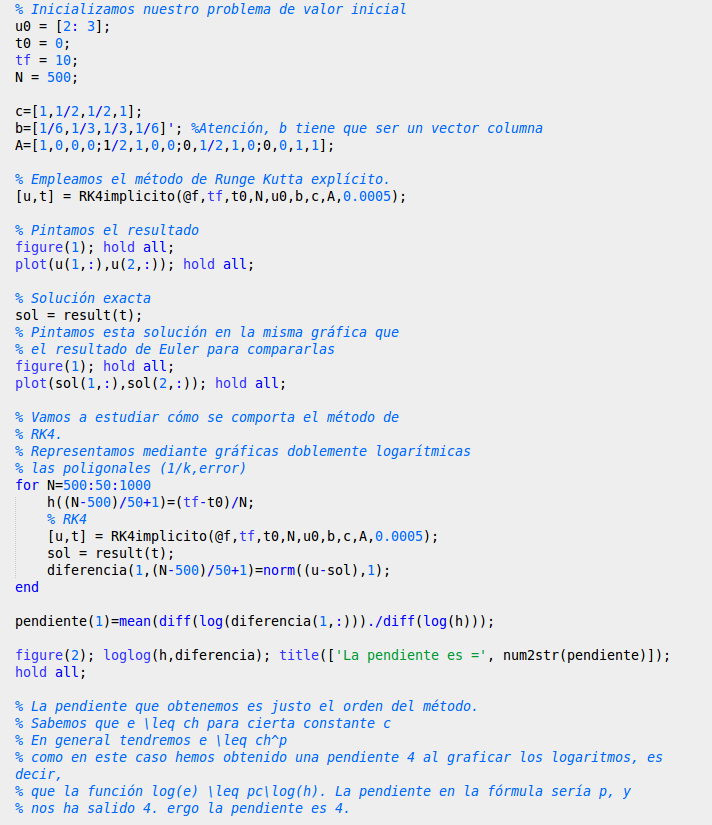
\includegraphics[width=0.6\textwidth]{img/PVI_RK4_implicito.png}
\end{center}

Y el propio método queda como sigue:
\begin{center}
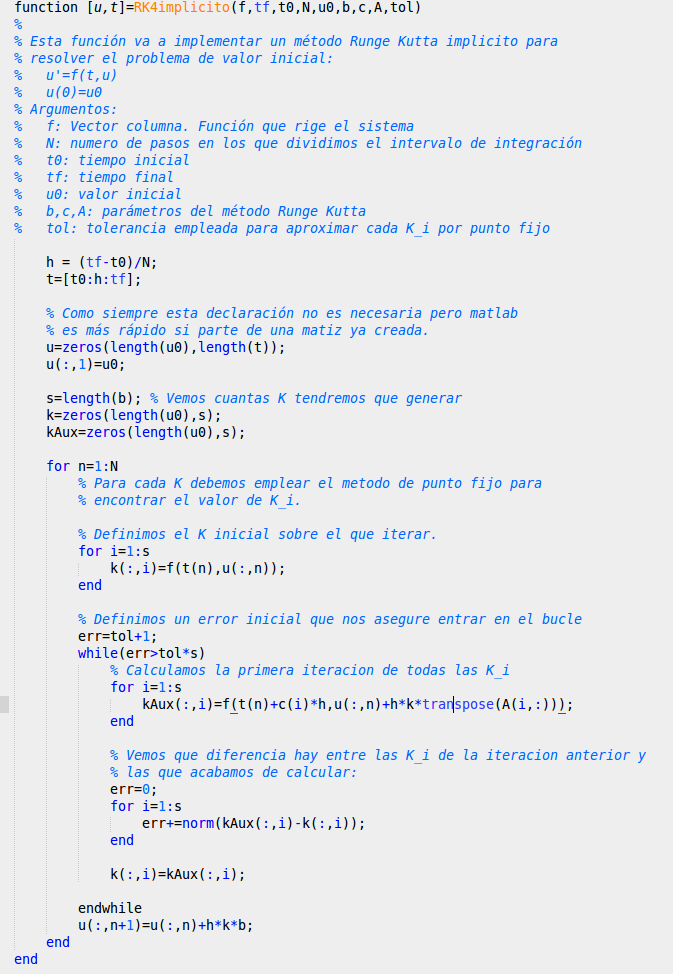
\includegraphics[width=0.6\textwidth]{img/RK4_implicito.png}
\end{center}

Finalmente, las gráficas obtenidas, que dibujan la función resultado y la obtenida con RK4 por un lado y la relación entre el erro y $h$ en escala logarítmica por otro, son:
\begin{center}
    \begin{minipage}{0.49\textwidth}
        \centering
        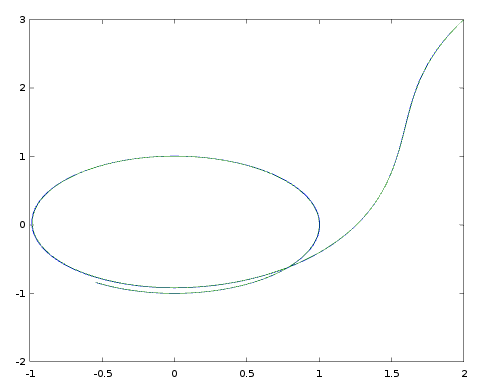
\includegraphics[width=\textwidth]{img/RK4_implicito_grafica.png}
    \end{minipage}
    \begin{minipage}{.49\textwidth}
        \centering
        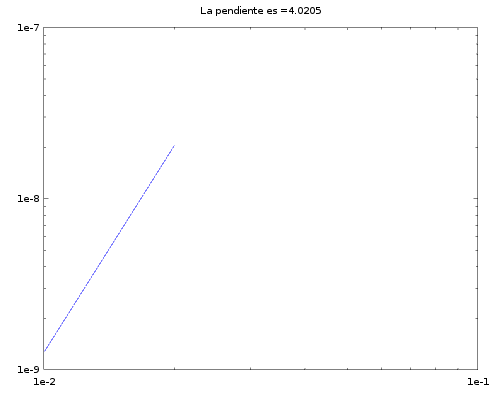
\includegraphics[width=\textwidth]{img/RK4_implicito_pendiente.png}
    \end{minipage}
\end{center}


\subsection{Método del trapecio}
Vamos a resolver una vez más el mismo PVI pero empleando esta vez el método del trapecio.

Para ello empezamos escribiendo una función que implemente dicho método:
\begin{center}
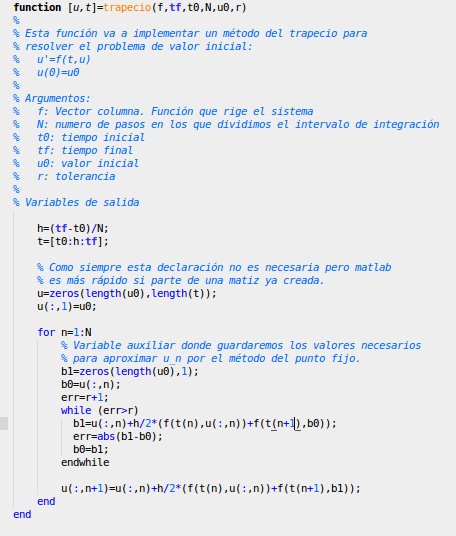
\includegraphics[width=0.6\textwidth]{img/trapecio.png}
\end{center}

La parte interesante de esta función se encuentra en el bucle while. El inconveniente del método del trapecio es que no es explícito, es decir, para calcular un $y_{n}$, la fórmula implica que necesitamos $y_n$.

La forma de resolver esto es aplicar el método del punto fijo para obtener una aproximación de $y_n$ y, a partir de esta aproximación, calcular el $y_n$ que nos da el método del trapecio.

Una vez tenemos el método implementado, reutilizamos las funciones $f$ y $resulto$ ya empleadas anteriormente y escribimos un pequeño programa que plantea el problema y lo resuelve incovando al método del trapecio.

\begin{center}
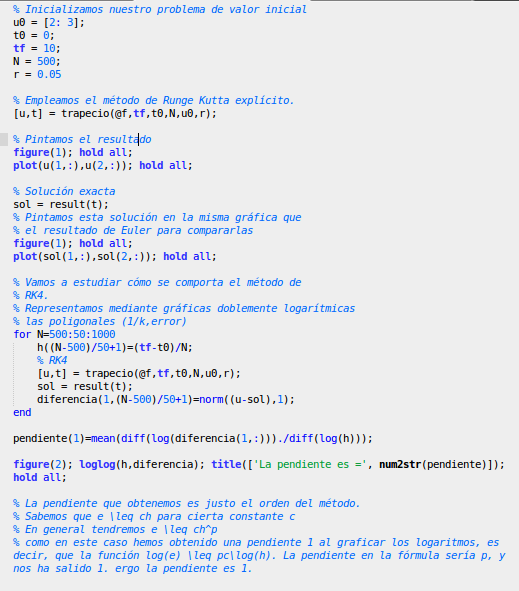
\includegraphics[width=0.6\textwidth]{img/PVI_trapecio.png}
\end{center}

Nuevamente, pintamos las gráficas de las funciones (la solución y la obtenida por el método numérico) para comprobar que coinciden y representamos el error respecto a $h$ en escala logarítmica para conocer la pendiente.

\begin{center}
    \begin{minipage}{0.49\textwidth}
        \centering
        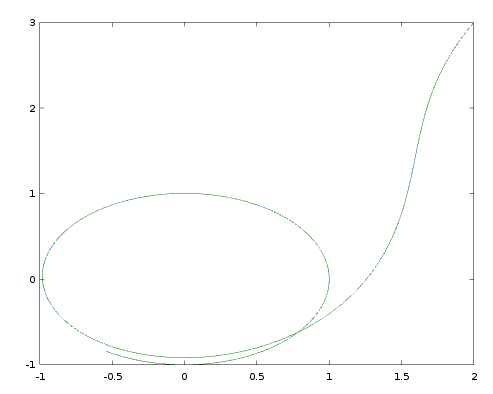
\includegraphics[width=\textwidth]{img/trapecio_grafica.png}
    \end{minipage}
    \begin{minipage}{.49\textwidth}
        \centering
        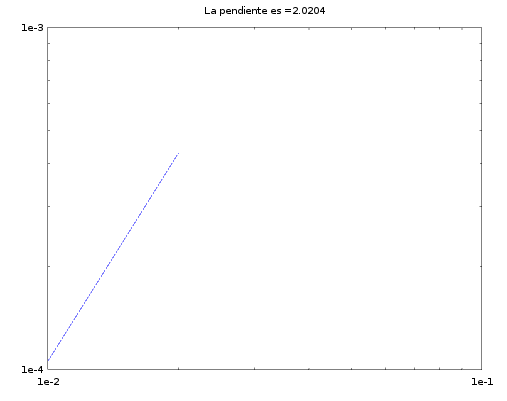
\includegraphics[width=\textwidth]{img/trapecio_pendiente.png}
    \end{minipage}
\end{center}

